\documentclass[../main.tex]{subfiles}
\begin{document}
\chapter{Hands-on Algorithmic Problem Solving}
The purpose of this chapter to see how our learned algorithm design principle can be applied into problem solving. We approach problems  using different algorithm design principle and step by step to see how the change in the time and space complexity. 

\paragraph{Longest Increasing Subsequence (300L)} Given an unsorted array of integers, find the length of longest increasing subsequence.
\begin{lstlisting}[numbers=none]
Example:

Input: [10,9,2,5,3,7,101,18]
Output: 4 
Explanation: The longest increasing subsequence is [2,3,7,101], therefore the length is 4. 
\end{lstlisting}
% \textit{Note: (1) There may be more than one LIS combination, it is only necessary for you to return the length. (2) Your algorithm should run in $O(n^2)$ complexity. Follow up: Could you improve it to $O(n\log  n)$ time complexity?}


% \textbf{Brute-force DFS.} Using the knowledge from DFS and backtracking, the subsequence is similar to the combination: for each element, it has two choice, either be used if it is larger than last element in the path or not be skipped. We can use the following DFS code to generate all possible LIS and obtain the maximum lenghth. This way, because it has two choice at each step to add the element or not, this makes it a binary tree, with the height of the tree to be n. And the worst time complexity is $O(2^n)$. 
% \begin{lstlisting}[language=Python]
% # DFS brute-force (using choice-tree)
% def subsequence(self, nums):
%     def dfs(idx, prev):
%         if idx == len(nums):
%             return 0
%         # choice one: use current element: [pre]+
%         taken = 0
%         if nums[idx] > prev:
%             taken = 1 + dfs(idx + 1, nums[idx])
%         # choice two: skip current element
%         not_taken = dfs(idx + 1, prev)              
%         return max(taken, not_taken)
% \end{lstlisting}
% However, the above solution makes it difficult to optimize with memoization, , as the solution it uses previous index and current index as keyes. because we have no sense of subproblems, it was simply doing search at the solution space.
\section{Direct Approach}
\subsection{Search in Graph}
In a subsequence, an item can only have two choice: either in or out of the resulting subsequence, this makes our total subsequence $O(2^n)$. As we know the searching process shall always be a search tree, we now start to generate this subsequence, which starts from \texttt{[]}. At the first level, we have item 10 that have two actions: not adding or adding, which makes it a two branches. At the second level, we consider item 9. This makes a search space of a binary tree, and we generate node implicitly since we only need to track the length of the path so far, and we need value of the last item to decide the children of current level. So far, we managed to model our problem as finding the longest path in the search tree, which is a binary tree and with height $n$. We can have the Python code:
\begin{lstlisting}[language=Python]
def lengthOfLIS(self, nums: List[int]) -> int:
    def dfs(nums, idx, cur_len, last_num, ans):
        if idx >= len(nums):
            ans[0] = max(ans[0], cur_len)
            return 
        if nums[idx] > last_num:
            dfs(nums, idx+1, cur_len + 1, nums[idx], ans)
        dfs(nums, idx+1, cur_len, last_num, ans)
    ans = [0]
    last_num = -sys.maxsize
    dfs(nums, 0, 0, last_num, ans)
    return ans[0]
\end{lstlisting}
\subsection{Self-Reduction}
 Now, let us us an example smaller than before, say [2, 5, 3, 7], which has the LIS 3 with [2, 3, 7]. Let us consider each state not atomic but as a subproblem. The same tree, but we translate each node differently. We start to consider the problem top down: we have problem [2, 5, 3, 7], and our start index = 0, meaning start from item 2, then our problem is can be divided into different situations:
\begin{itemize}
    \item not take 2: we find the LIS length of subproblem [5, 3, 7]. In this case, our subsequence can start from any of these 3 items, we indicate this case by not changing the previous value. Use \texttt{idx} to indicate the subproblem/subarray, we call dfs that \texttt{idx+1}. 
    \item take 2: we need to find  the LIS length of subproblem [5, 3, 7] whose subsequence must start from 5. Thus, we set the \texttt{last\_num} to 5 in the recursive call.  
\end{itemize}
Therefore, our code becomes: 
\begin{lstlisting}[language=Python]
def lengthOfLIS(self, nums: List[int]) -> int:
    def dfs(nums, idx, last_num):
        if not nums:
            return 0
        if idx >= len(nums):
            return 0
        len1 = 0
        if nums[idx] > last_num:
            len1 = 1 + dfs(nums, idx+1, nums[idx])
        len2 =  dfs(nums, idx+1, last_num)
        return max(len1, len2)
    
    last_num = -sys.maxsize
    return dfs(nums, 0, last_num)
\end{lstlisting}
In this solution, the time complexity has not improved yet, but from this approach, we can further increase the efficiency with dynamic programming. 
% In the example of  Fibonacci Sequence, we discussed four steps to come out with a bottom-up tabulation dynamic programming solution and the key words of each step is highlighted with italic -- state, initialization, recurrence function, and answer. With the example of longest increasing subsequence (LIS), we would further enhance the comparison of complete search with dynamic programming and the tabulation method with the step of formulating the recurrence relation (or state transfer function) by ourselves.

% \textit{Note: (1) There may be more than one LIS combination, it is only necessary for you to return the length. (2) Your algorithm should run in $O(n^2)$ complexity. Follow up: Could you improve it to $O(n\log  n)$ time complexity?}


\subsection{Dynamic Programming}
\paragraph{Memoization} We have known that the recurrence relation takes $LIS(i, prev) = max(LIS(i+1, prev), LIS(i+1, nums[i])$. How many possible states for $LIS(i, prev)$? $i \in [0, n-1]$, and $prev$ can have $n$ candidates too, this makes the whole state space only $n^2$. While, using the depth-first tree search we revisited a state multiple times, which eventually make the time complexity to $O(2^n)$. Now, let us modify the approach and use \texttt{memo} which is a dictionary and takes a tuple \texttt{(i, prev)} as key. If we found the state is not computed, we compute as we do in the previous implementation, if it exists in the memory, however, we just directly return the value and avoid recomputing again:
\begin{lstlisting}[language=Python]
def lengthOfLIS(self, nums: List[int]) -> int:
    def dfs(nums, idx, last_num, memo):
        if idx >= len(nums):
            return 0
        if (idx, last_num) not in memo:
            len1 = 0
            if nums[idx] > last_num:
                len1 = 1 + dfs(nums, idx+1, nums[idx], memo)
            len2 =  dfs(nums, idx+1, last_num, memo)
            memo[(idx, last_num)] = max(len1, len2)
        return memo[(idx, last_num)]
    
    last_num = -sys.maxsize
    memo = {}
    return dfs(nums, 0, last_num, memo)
\end{lstlisting}




\section{A to B} Another approach is to use the concept of ``prefix'' or ``suffix''. The LIS must start from one of the items in the array. Finding the length of the LIS in the original array can be achieved by comparing n subproblems, the length of LIS of:
\begin{lstlisting}
[2, 5, 3, 7], LIS starts at 2,
[5, 3, 7], LIS starts at 5, 
[3, 7], LIS starts at 3
[7], LIS starts at 7
\end{lstlisting}
\subsection{Self-Reduction} 
We model the problem as in Fig.~\ref{fig:tree_lis}. 
\begin{figure}[h]
    \centering
    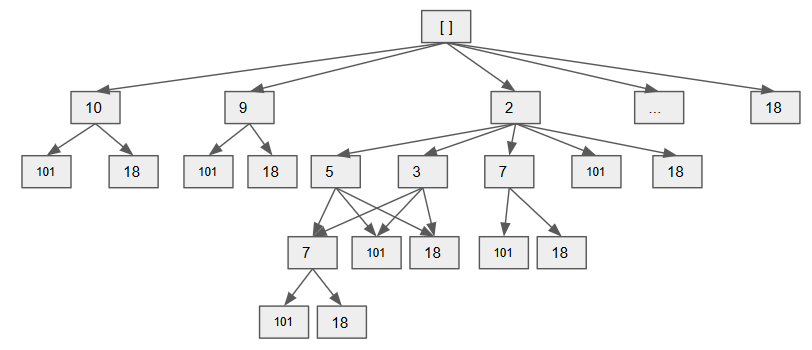
\includegraphics[width=0.8\columnwidth]{fig/LIS_tree.png}
    \caption{Graph Model for LIS, each path represents a possible solution. %Each arrow represents an move: find an element in the following elements %that's larger than the current node.
    }
    \label{fig:tree_lis}
\end{figure}
Same here, our problem become finding the longest path in a N-ary tree instead of a binary tree. Define $f(i)$ as the LIS starting with index $i$ in the array. then, its relation with other state will be $f(i) = \max_j(f(j))+1, j>i$, $a[j]>a[i]$, and $f[n]=0$. Here, the base case is when there has element to start from which will have 0 LIS. 
\begin{lstlisting}[language=Python]
def lengthOfLIS(self, nums: List[int]) -> int:
    def dfs(nums, idx, cur_num):
        max_len = 0
        # Generate the next node
        for i in range(idx+1, len(nums)):
            if nums[i] > cur_num:
                max_len = max(max_len, 1 + dfs(nums, i, nums[i]))
        return max_len
    return dfs(nums, -1, -sys.maxsize)
\end{lstlisting}
\subsection{Dynamic Programming} 
\paragraph{Memoization} Similar to the last approach, we can write code:
\begin{lstlisting}[language=Python]
def lengthOfLIS(self, nums: List[int]) -> int:
    def dfs(nums, idx, cur_num, memo):
        max_len = 0
        # Generate the next node
        if (idx, cur_num) not in memo:
            for i in range(idx+1, len(nums)):
                if nums[i] > cur_num:
                    max_len = max(max_len, 1 + dfs(nums, i, nums[i], memo))
            memo[(idx, cur_num)] = max_len
        return memo[(idx, cur_num)]
    memo = {}
    return dfs(nums, -1, -sys.maxsize, memo)
\end{lstlisting}
\paragraph{Tabulation}  With the bottom-up manner, we need to tweet our above recurrence function and definition of state. The subproblem $f(i)$ here will be defined as the LIS ending at index $i$. We shall pay attention that with $n$ elements there should exist $n+1$ states in total, that there is an empty state with empty array $[]$. The recurrence function will be shown in Eq.~\ref{LIS_equation}. It can be explained the LIS ending at index $i$ will be transitioned from LIS ending at any previous index by plusing one.  The whole analysis process is illustrated in Fig~\ref{fig:lis}.    
\begin{equation}
\label{LIS_equation}
    f(i) = \begin{cases}
    1 + max(f(j)),& -1\leq j<i < n, arr[j] < arr[i];\\
    0& \text{i=-1}
    \end{cases}
\end{equation}
\begin{figure}[!ht]
    \centering
    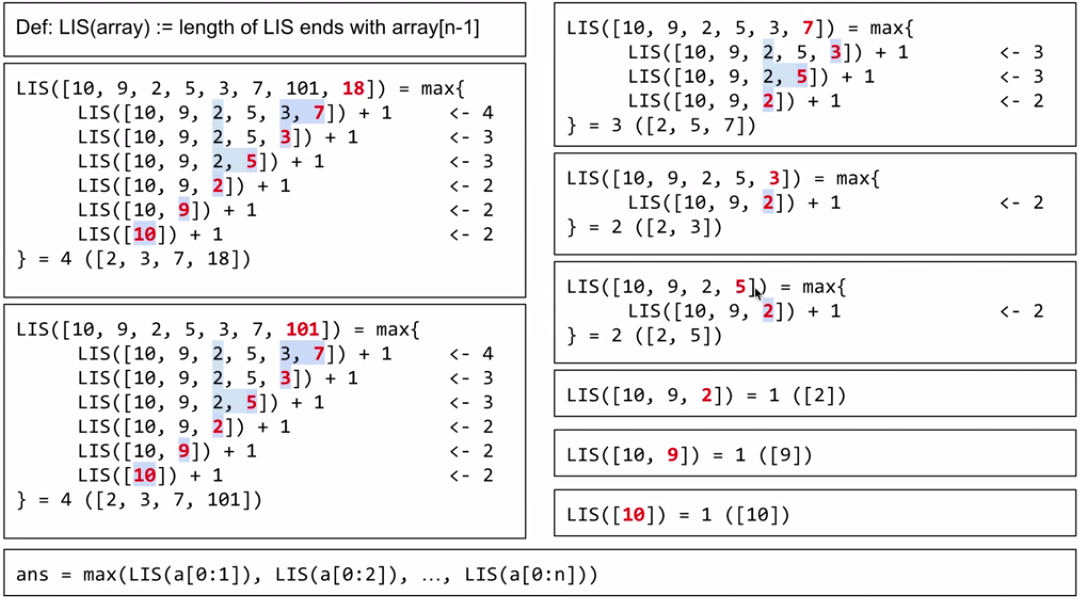
\includegraphics[width=0.8\columnwidth]{fig/LIS.png}
    \caption{The solution to LIS. }
    \label{fig:lis}
\end{figure}
To simply the implementation, we insert a $-\infty$ value at the beginning of the array. To initialize we set $dp[0] = 0$, and the answer is $max(dp)$.  The time complexity is $O(n^2)$ because we need two for loops: one outsider loop with $i$, and another inside loop with $j$. The space complexity is $O(n)$. The Python code is:
\begin{lstlisting}[language= Python]
def lis(a):
  # define the dp array
  dp = [0] * (len(a)+1)
  a = [-sys.maxsize] + a
  print(a)
  for i in range(len(a)): # end with index i-1
    for j in range(i):
      if a[j] < a[i]:
        dp[i] = max(dp[i], dp[j] + 1)
  print(dp)
  return max(dp)
\end{lstlisting}
\subsection{Divide and Conquer}
We can even speedup further by using binary search, the second loop we can use a binary search to make the time complexity $O(logn)$, and the dp array used to save the maximum ans. Each time we use binary search to find an insertion point, if it is at the end, then the length grow.
[4]->[4,10],->[4,10],[3,10],->[3,8]->[3,8,9]
\begin{lstlisting}[language = Python]
def lengthOfLIS(self, nums):
        """
        :type nums: List[int]
        :rtype: int
        """
        def binarySearch(arr,l,r,num):
            while l<r:
                mid = l+(r-l)//2
                if num>arr[mid]:
                    l=mid+1
                elif num<arr[mid]:
                    r=mid
                else:
                    return mid
            return l
        max_count = 0
        if not nums:
            return 0
        dp =[0 for _ in range(len(nums))]#save the maximum till now
        maxans =1
        length=0
        for idx in range(0,len(nums)): #current combine this to this subsequence, 10 to [], 9 to [10]
            pos = binarySearch(dp,0,length,nums[idx]) #find insertion point
            dp[pos]= nums[idx] #however if it is not at end, we replace it, current number
            if pos==length:
                length+=1
        print(dp)            
        return length
\end{lstlisting}
% Note: dp array does not result in longest increasing subsequence, but length of dp array will give you length of LIS. A dynamic demo can be found here: https://en.wikipedia.org/wiki/Longest\_increasing\_subsequence
% \#/media/File:LISDemo.gif. The code:
\begin{lstlisting}[language=Python]
    def lengthOfLIS(self, nums):
        """
        :type nums: List[int]
        :rtype: int
        """
        def binarySearch(arr,l,r,num):
            while l<r:
                mid = l+(r-l)//2
                if num>arr[mid]:
                    l=mid+1
                elif num<arr[mid]:
                    r=mid
                else:
                    return mid
            return l
        max_count = 0
        if not nums:
            return 0
        dp =[0 for _ in range(len(nums))]
        LIS=0
        for i in range(len(nums)): #current combine this to this subsequence, 10 to [], 9 to [10]
            pos = binarySearch(dp,0,length,nums[i])
            dp[pos]= nums[i]
            if pos==LIS:
                LIS += 1          
        return LIS
\end{lstlisting}
\end{document}